%Templated from IEEE Preparation Papers
\documentclass[letterpaper, 10 pt, conference]{ieeeconf}

\IEEEoverridecommandlockouts                              % This command is only
                                                          % needed if you want to
                                                          % use the \thanks command
\overrideIEEEmargins
% See the \addtolength command later in the file to balance the column lengths
% on the last page of the document



%The following packages can be found on http:\\www.ctan.org
\usepackage{graphics} % for pdf, bitmapped graphics files
\usepackage{epsfig} % for postscript graphics files
\usepackage{mathptmx} % assumes new font selection scheme installed
\usepackage{times} % assumes new font selection scheme installed
\usepackage{amsmath} % assumes amsmath package installed
\usepackage{amssymb}  % assumes amsmath package installed



\title{\LARGE \bf
Globally Asynchronous Locally Synchronous Processing
}

\author{ \parbox{3 in}{\centering Will Wu\\
        Electrical and Computer Engineering\\
        University of Rochester\\
        500 Computer Studies Building \\
        Rochester, NY 14627\\
        {\tt\small ywu37@ur.rochester.edu}}
}

\begin{document}



\maketitle
\thispagestyle{empty}
\pagestyle{empty}


%%%%%%%%%%%%%%%%%%%%%%%%%%%%%%%%%%%%%%%%%%%%%%%%%%%%%%%%%%%%%%%%%%%%%%%%%%%%%%%%
% \begin{abstract}


% \end{abstract}


%%%%%%%%%%%%%%%%%%%%%%%%%%%%%%%%%%%%%%%%%%%%%%%%%%%%%%%%%%%%%%%%%%%%%%%%%%%%%%%%

\section{THE ANATOMY OF DIGITAL SIGNALS}

Conventional electronics derive its energy from an analog voltage source.  Devices called analog to digital converters assigns ranges of analog voltages to specific digital voltage levels.  This voltage source can be divided into the simplest of these delineations: that of two voltage levels (high voltage and low voltage) which allows for the use of boolean algebra.  Digital signals are the foundation of hardware that allows for computing.  As such, the computer is developed to handle binary logic.  


There are many aspects of state transition that must be carefully accounted for as unaccounted for behaviors during state transitions is the primary cause of incorrect device operation.  Set up time is the amount of time a signal must remain before a clock's state transition to ensure accurate reading of the line.  This is to account for the latencies associated with the resolution of values in the data.  An attempt is made in design to eliminate On the other side of the relevant clock edge, the signal must be stable after a clock's state transition to ensure accurate latching.  If not enough time is dedicated to abiding by set up time and hold time parameters, this may result in data corruption.

Slew is defined as the rate that a signal switches from one logic state to a different logic state.  This is computed as the reciprocal of time so this value can never be undefined as we modeling state transitions as simultaneous would invalidate the rest of this paper.

Propagation delay is defined as the latency between the time a signal change is realized on another signal (such as the input of a logic gate to the output of that logic gate).  The period is the duration for a signal to complete one cycle.  For the purposes of this paper, the period of the clock signal is essential to the design process.  If the propagation delay of the clock signal through the network extends longer than one clock period, invalid operations may occur as some processing cores may be idle when supposed to be working or vice versa.  Phase is thought of as the relative displacement between two signals.  Another way of thinking about phase is the fraction of the period one signal is in relation to the start of one period of the other signal.  Signals are said to be synchronous when the period among signals is identical.


\begin{equation}
Frequency = \frac{(V_{dd}-V_t)^{\alpha}}{V_{dd}} \\
\end{equation}

\section{GENERATING THE CLOCK SIGNAL}

As conventional designs have increased the clock frequency, the running of this system dissipates immense power.  We can roughly calculate the power dissipated from the clock signal itself with the following formula:

\begin{equation}
Power = Capacitance * Voltage ^2 * frequency \\
\end{equation}

It follows that as the device clock frequencies have increased, so have the heat dissipation cost of processing.  So it is not particularly efficient to consistently run a high frequency clock only to have periods of idle processing cores.  With a clock divider, one can dictate if a processor is working or idle.  Idle processors have their clock frequencies set to the global clock frequency.  With different loads assigned to different processing cores, one may have cores run at different clock frequencies. is to have clocks be rational multiples of one another.  Lastly, the voltage contribution to the power dissipation minimization problem can also be adjusted.  The analog voltage amplitude may be lowered during  periods of processor idling.


A locally generated clock is constructed from a ring oscillator which consist of a series of NOT gates in a ring network with a NAND gate to control clock pausing.  Circuitry that controls whether or not to generate the next clock pulse as well as its frequency is called the clock arbiter.  Each connection to neighboring nodes is assigned to a mutex and all mutexes must be in agreement in order for the next clock pulse to happen.  The local clock can be stretched with the use of the adjustable delay line.  The stretching factor $\alpha$ has a lower limit of 0 in the case of long clock cycle and an upper limit of half the clock period.

Conflicts may arise during clock generation such that the relevant state transition in the clock coincides too closely with a change with regards to incoming data from a different node.  As discussed before, this means that data corruption can be possible due to setup time and hold time not being satisfied.  This is where the clock can be artificially slowed through the use of the strech factor.  Another simple solution is to offset the data state changes slightly.  The hold time can be shortened by adding a buffer on the write request lines, thus delaying mutex latching.


%Stoppable clock generation
\begin{figure}[!ht] %
	\centering
	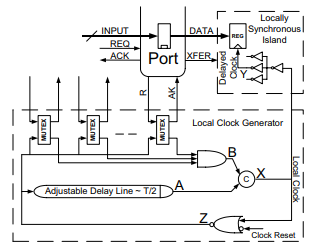
\includegraphics [width=0.5\textwidth] {Clock_Generation.PNG} 
    \caption{The circuit logic for generating local clock signals and accepting ports. [6]}

\end{figure}

\begin{figure}[!ht] %
	\centering
	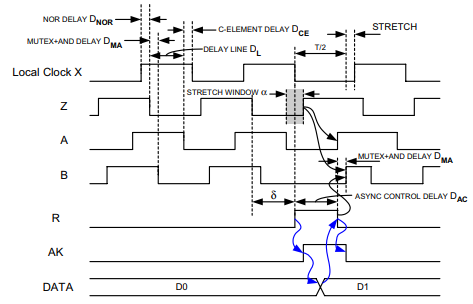
\includegraphics [width=0.5\textwidth] {Wave_Diagram_Clock_Generation.PNG} 
    \caption{The wave diagram for the clock generation circuit. [6]}
\end{figure}

With all clock synchronization designs, control skew must be strictly enforced as differing skews can easily result in asynchronization.

\section{WORKING ASYNCHRONOUSLY}

\begin{figure}[!ht] %
	\centering
	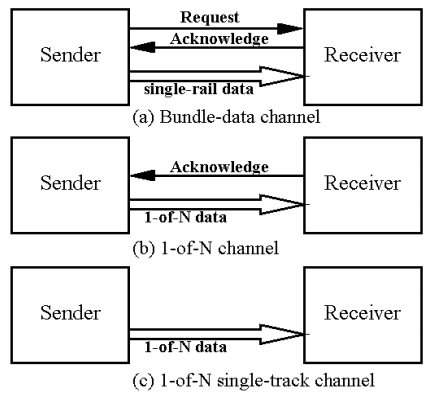
\includegraphics [width=0.5\textwidth] {Asyc_Channel.PNG} 
    \caption{The three different types of asynchronous node to node communication. [3]}
\end{figure}

Most asynchronous designs use handshaking between two nodes to maintain consistency.[3]  The process involves a sender and a receiver sending acknowledgement (ACK) or non acknowledgement (NACK) messages between each other.  This allows for the sender and receiver to operate on different clock periods.  After request and acknowledgement that data can be transferred, there are three methods of transferring that data.  The conventional single-rail data channel allocates one wire per one data stream.  Another method of data transfer is with 1 to N channels.  This assigns N data wires to send $log_2N$ bits of data. Lastly, method of data transfer that is not sensitive to delay and does not require ACK/NACK messages is the single-track channel in which the sender sends data to the receiver in one continuous stream.  This method is possible if the receiving buffer is adequately large.

\begin{figure}[!ht] %
	\centering
	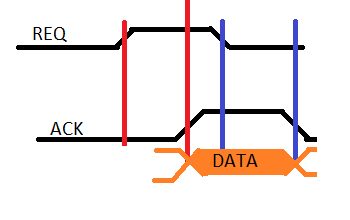
\includegraphics [width=0.5\textwidth] {Data_Transfer.png} 
    \caption{The timing diagram of data transfer through request and acknowledgement tokens.}
\end{figure}

For a different method of computing data receiver is to design a centralized arbiter.  The group of Bertozzi et al. proposed an arbitration unit consisting of a 2-way root bisection hierarchy with flattened tree.  This allows for short length data travel at the expense of low bisection bandwidth.


\begin{figure}[!ht] %
	\centering
	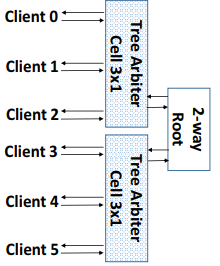
\includegraphics [width=0.5\textwidth] {Tree_Arbiter.PNG} 
    \caption{Fat tree arbitration in asynchronous systems.[5]}
\end{figure}


\section{CASE STUDY: BAUGH WOOLEY MULTIPLIER}

Multiplication computations utilize multistage Booth's algorithm or a series of add-shift operations so they are known to take many clock cycles.  The team of Wazurkar et al. proposed a 16-bit multiplier using the Baugh Wooley algorithm and the GALS model implemented on an FPGA.  This algorithm handles sign of partial products at every step of the process.  The mesh network is shown below with 'a' lines corresponding to the bits of one operand and the 'b' lines corresponding to the bits of the other operand.  The algorithm allows for pipelining through the network from top to bottom.  The enable lines are what drives the datagrams from one stage to the next.

The global clock frequency is slowed down and divided among the number of stages in the pipeline.  This allows for the throughput to remain the same as that of a global clock setup.  A global clock setup effectively has all processing cores fed the high frequency clock signal.  In comparison, the design with the clock divider allows for idle processing cores to not be enabled and as a result, dissipate less power.  This is at the expense of more circuitry with the GALS design taking up 106\% more slice LUTs. [2]

\begin{figure}[!ht] %
	\centering
	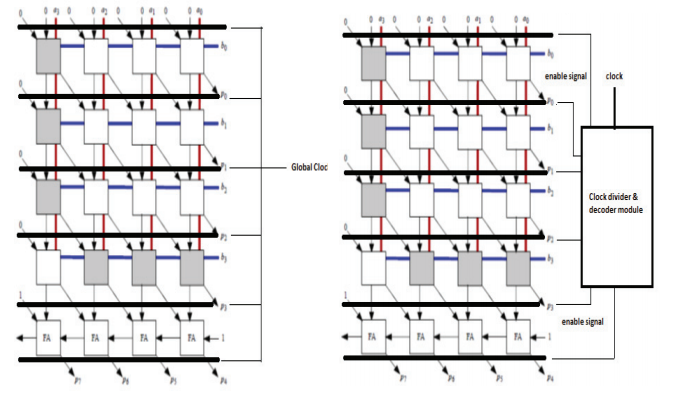
\includegraphics [width=0.5\textwidth] {Multiply_Network.png} 
    \caption{Baugh Wooley multiplier processor array.}
\end{figure}

\begin{figure}[!ht] %
	\centering
	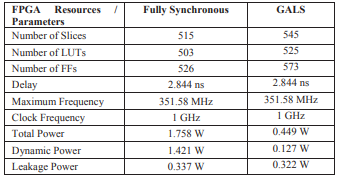
\includegraphics [width=0.5\textwidth] {Multiply_Results.PNG} 
    \caption{The evaluation of power dissipation for the Baugh Wooley multiplier.}
\end{figure}

\section{CASE STUDY: AN ASYNCHRONOUS ARRAY OF SIMPLE PROCESSORS}

The group of Zhiyi Yu et al. at the University of California Davis present a multicore processor specifically designed for digital signal processing applications.  They call it The Asynchronous Array of Simple Processors (AsAP).  The multiple cores are arranged in a two dimensional 6 by 6 mesh network.  Data enters through one end of the mesh array and exits on the other end of the mesh array.  Each AsAP processor has its own clocking system with clock oscillator with a divider of up 128.  The processors communicate with their respective next-door neighbor using dual clock FIFO queues.  The apparatus can select input from each of its cardinal neighbors and can output to each of its cardinal neighbors.  The synchronization mechanism is found with the gray/binary address conversion and computation.  Overall, the group found that its design was 14 times more energy efficient than other processors and uses 66\% more of its area for the processor. [4]

\begin{figure}[!ht] %
	\centering
	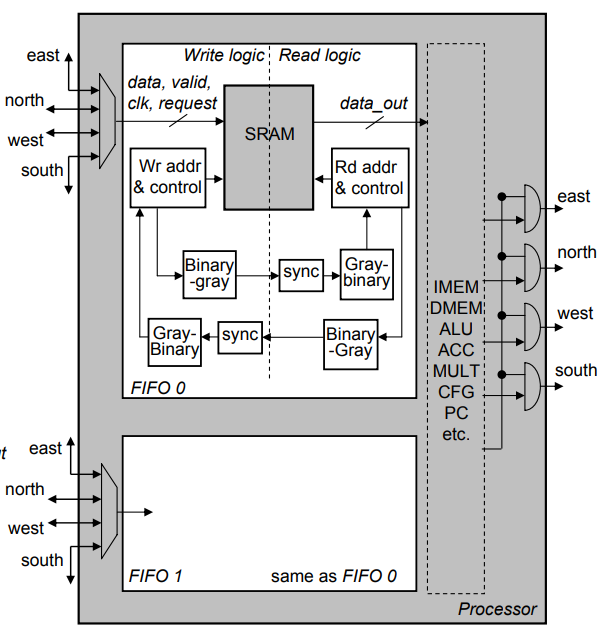
\includegraphics [width=0.5\textwidth] {Node_IO.PNG} 
    \caption{The schematic diagram of the synchronization and communications logic for the AsAP processor. [4]}
\end{figure}

\section{FINAL REMARKS}

The increase in number of processing core on a chip does not appear to be stopping anytime soon.  And with that trend, the expectations of a large chip working synchronously to a high frequency clock intended for all cores does not account for the time it takes for electrical signals to traverse through the long distances of wiring on current chip designs.  Development in clock generation is quite difficulty to be sure.  Much of the issue arises in the development phase with software simulator models being too idealistic with regards to timing.  Arbiters and synchronizers are by design nondeterministic and so design validation using software is very complicated.  Validation software and novel designs of research groups will need to improve in tandem so that the rate of development in this field increases.

\addtolength{\textheight}{-12cm}   % This command serves to balance the column lengths
                                  % on the last page of the document manually. It shortens
                                  % the textheight of the last page by a suitable amount.
                                  % This command does not take effect until the next page
                                  % so it should come on the page before the last. Make
                                  % sure that you do not shorten the textheight too much.


\begin{thebibliography}{99}

\bibitem{c1} D.M. Chapiro, Globally-Asynchronous Locally-synchronous Circuits, Ph.D. diss., Stanford University, U.S.A., Oct., 1984. 

\bibitem{c2} G. Wazurkar and S. L. Badjate, "Globally asynchronous locally synchronous (GALS) pipelined signed multiplier," 2016 International Conference on Computing, Analytics and Security Trends (CAST), Pune, 2016, pp. 383-386.

\bibitem{c4}  Y. Zhiyi et al., "An Asynchronous Array of Simple Processors For DSP Applications," Proc. Int’l Solid-State Circuits Conf Dig. Tech. Papers (ISSCC 06), IEEE Press, 2006,
pp. 428-429.

\bibitem{c3} Peter A. Beerel: Asynchronous Circuits: An increasingly practical design solution. Proceedings of ISQED'02, IEEE Computer Society (2002)

\bibitem{c5} D. Bertozzi, G. Miorandi, M. Tala and S. M. Nowick, "Cost-Effective and Flexible Asynchronous Interconnect Technology for GALS Networks-on-Chip," 2017 New Generation of CAS (NGCAS), Genova, 2017, pp. 77-80.

\bibitem{c6} R. Dobkin, R. Ginosar and C. P. Sotiriou, "Data synchronization issues in GALS SoCs," 10th International Symposium on Asynchronous Circuits and Systems, 2004. Proceedings., 2004, pp. 170-179.

\bibitem{c7} X. Guan, D. Zhou, D. Wang, Y. Yang and Z. Zhu, "A Novel GALS Single-Track Protocol Asynchronous Communication Circuits," 2009 Pacific-Asia Conference on Circuits, Communications and Systems, Chengdu, 2009, pp. 269-272.

\end{thebibliography}

\end{document}


Sum count: 1747
Words in text: 1632
Words in headers: 32
Words outside text (captions, etc.): 79
Number of headers: 8
Number of floats/tables/figures: 8
Number of math inlines: 2
Number of math displayed: 2
